\subsection{Election November 3, 1908: *Taft vs Bryan}
\begin{frame}[t]{Election November 3, 1908: *William Taft}
\small
% Taft
\begin{columns}[T, onlytextwidth]
\column{0.48\textwidth}
\vspace{-1em}
{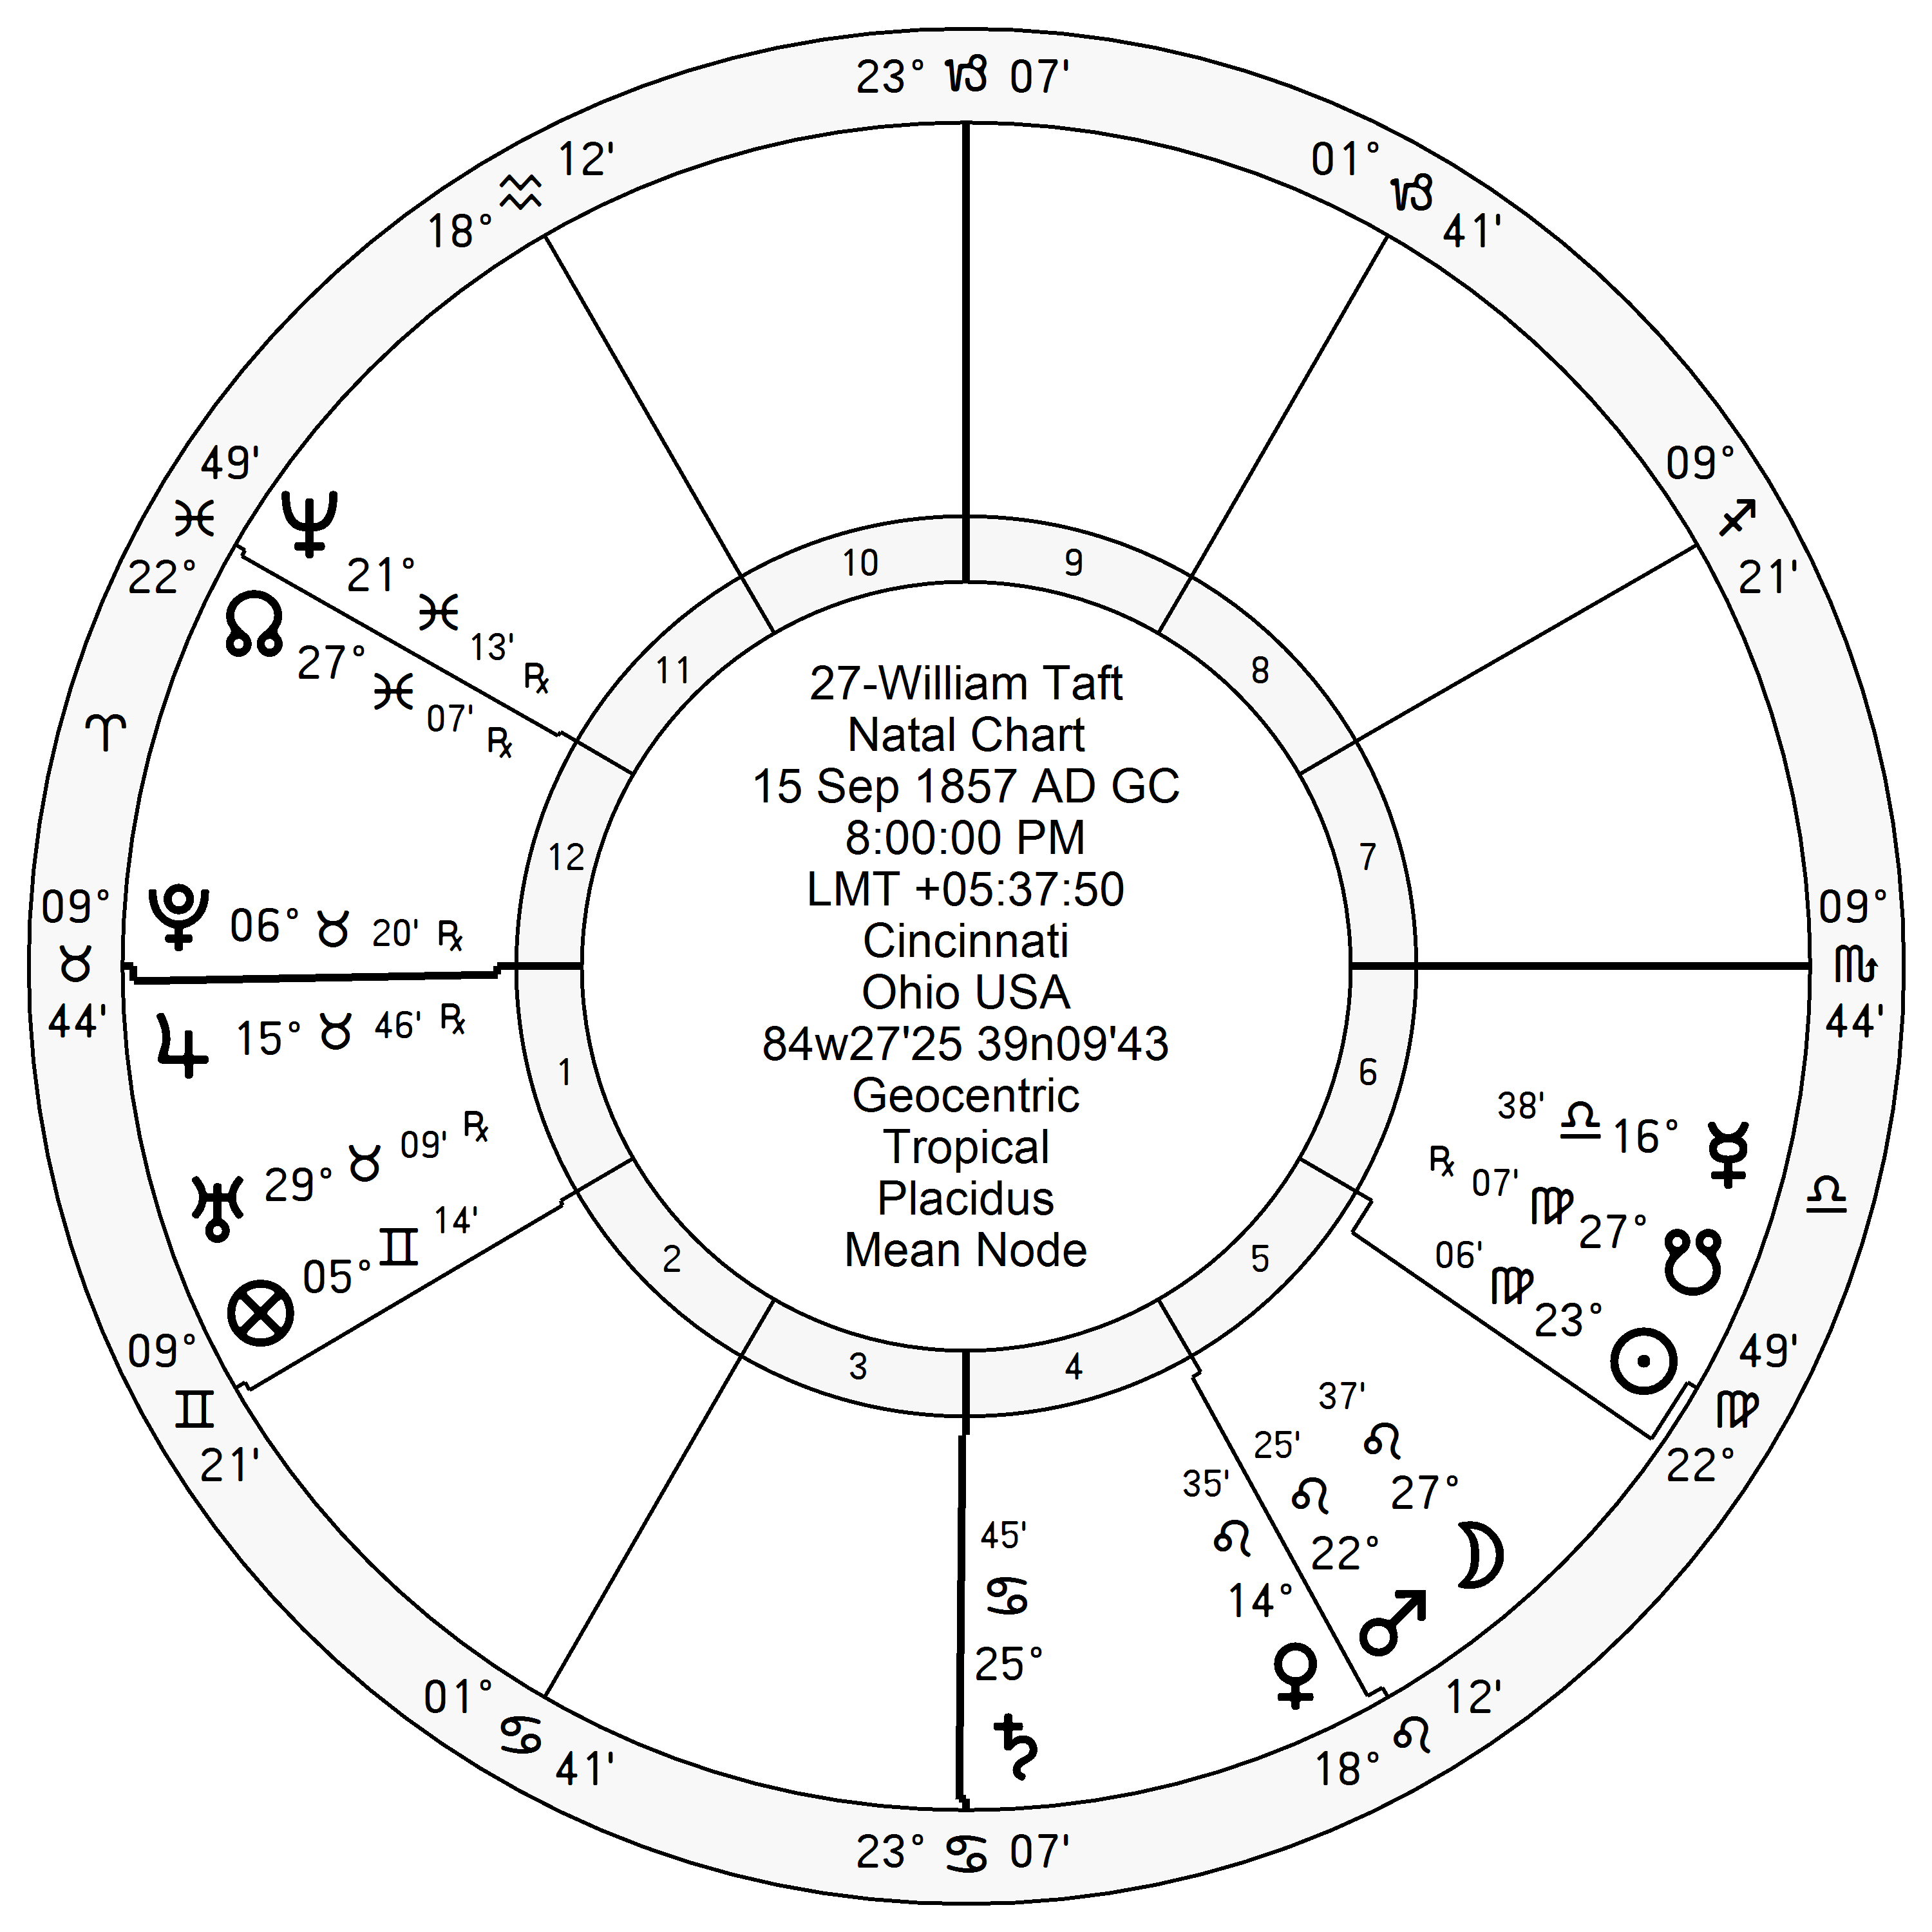
\includegraphics[width=0.9\textwidth]{charts/Taft.png}}
\fontsize{7pt}{8pt}\selectfont

There are connections between P1, P10 and N1 although the underlying houses are weak it appears Bryan's were weaker and worse. The \Sun\, with the \SouthNode\, may have marked him as a one term President.

\column{0.48\textwidth}
\vspace{-1em}
{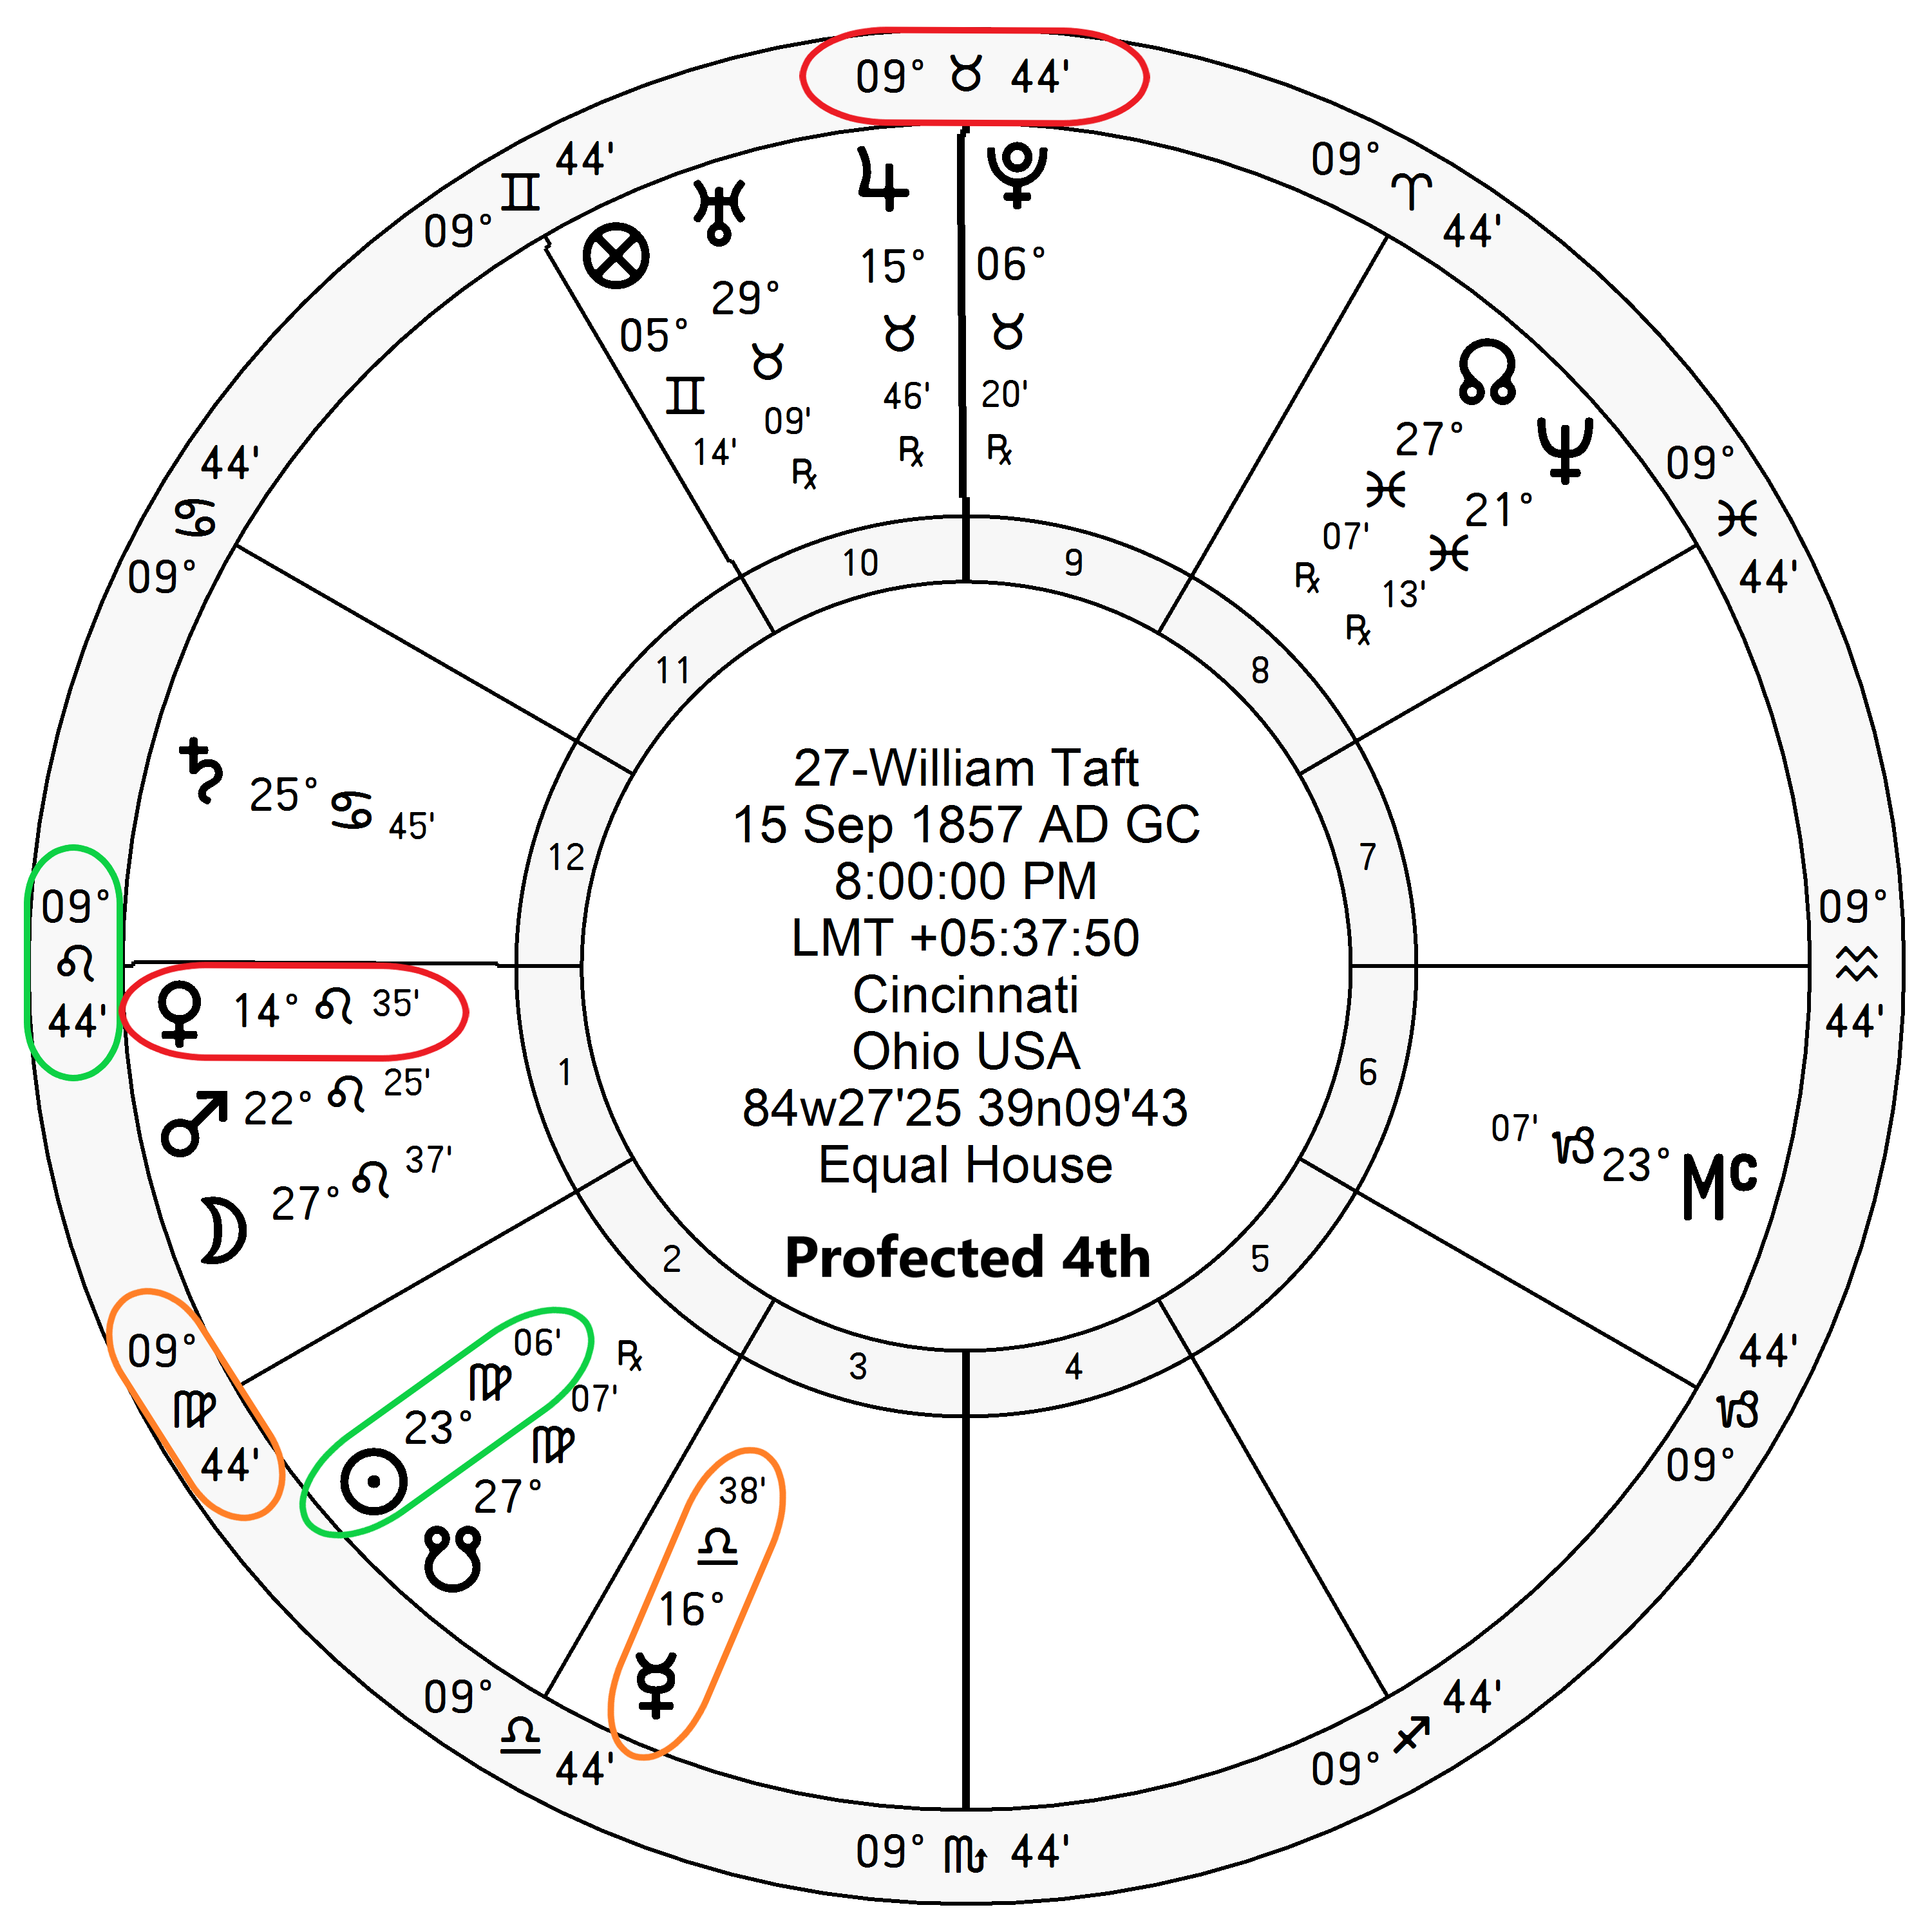
\includegraphics[width=0.9\textwidth]{charts/Taft-Prof-4th.png}}

\textbf{\dgreen P1}=N5
	$\Rightarrow$ \Sun\,\Conjunction\,\SouthNode $\Rightarrow$ \textbf{\dgreen P2/N6} \\
\textbf{\red P10=N1} 
	$\Rightarrow$  \Venus\, $\Rightarrow$  \textbf{\dgreen P1}/N4 \\
PE=\textbf{\dgreen P2/N6}
	$\Rightarrow$  \Mercury\, $\Rightarrow$  P3/\textbf{\dgreen N6}

\end{columns}
\end{frame}

% Bryan
\begin{frame}[t]{Election November 3, 1908: William Jennings Bryan}
\small
\begin{columns}[T, onlytextwidth]
\column{0.48\textwidth}
\vspace{-1em}
{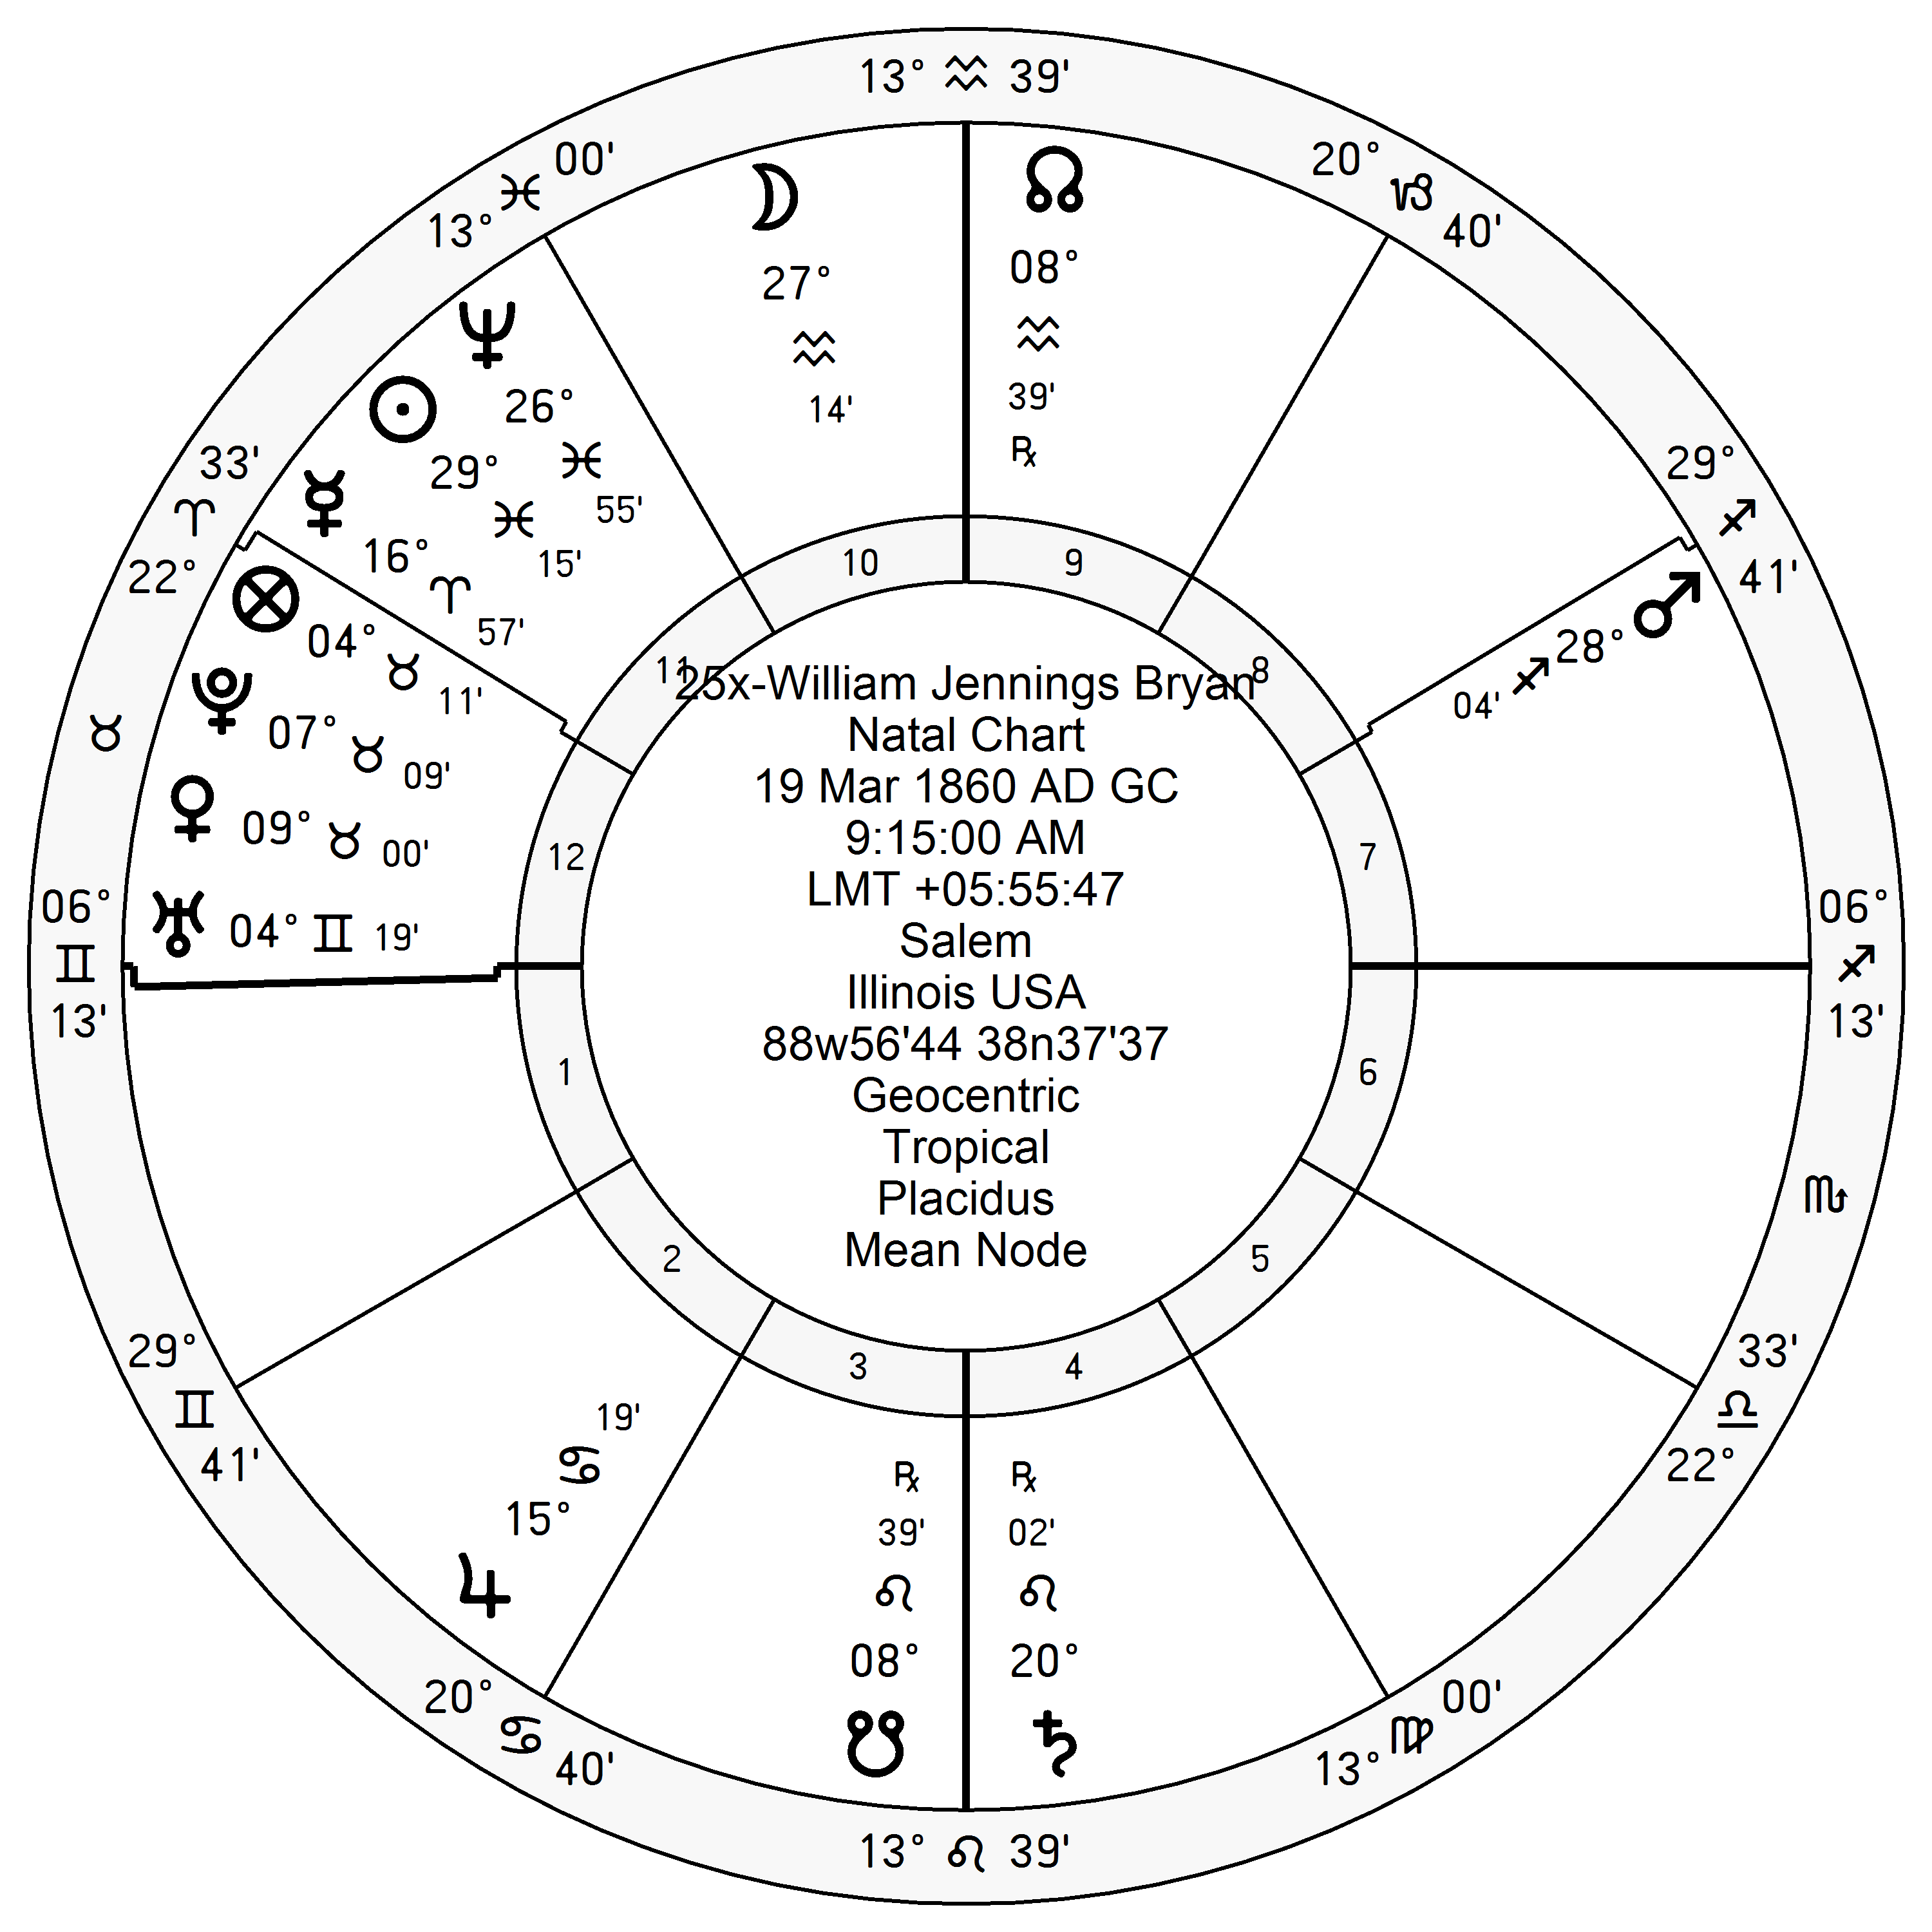
\includegraphics[width=0.9\textwidth]{charts/Bryan.png}}
\fontsize{8pt}{9pt}\selectfont

This election is 12 years to the day from the 1896 election; the setup and result are the same.

\column{0.48\textwidth}
\vspace{-1em}
{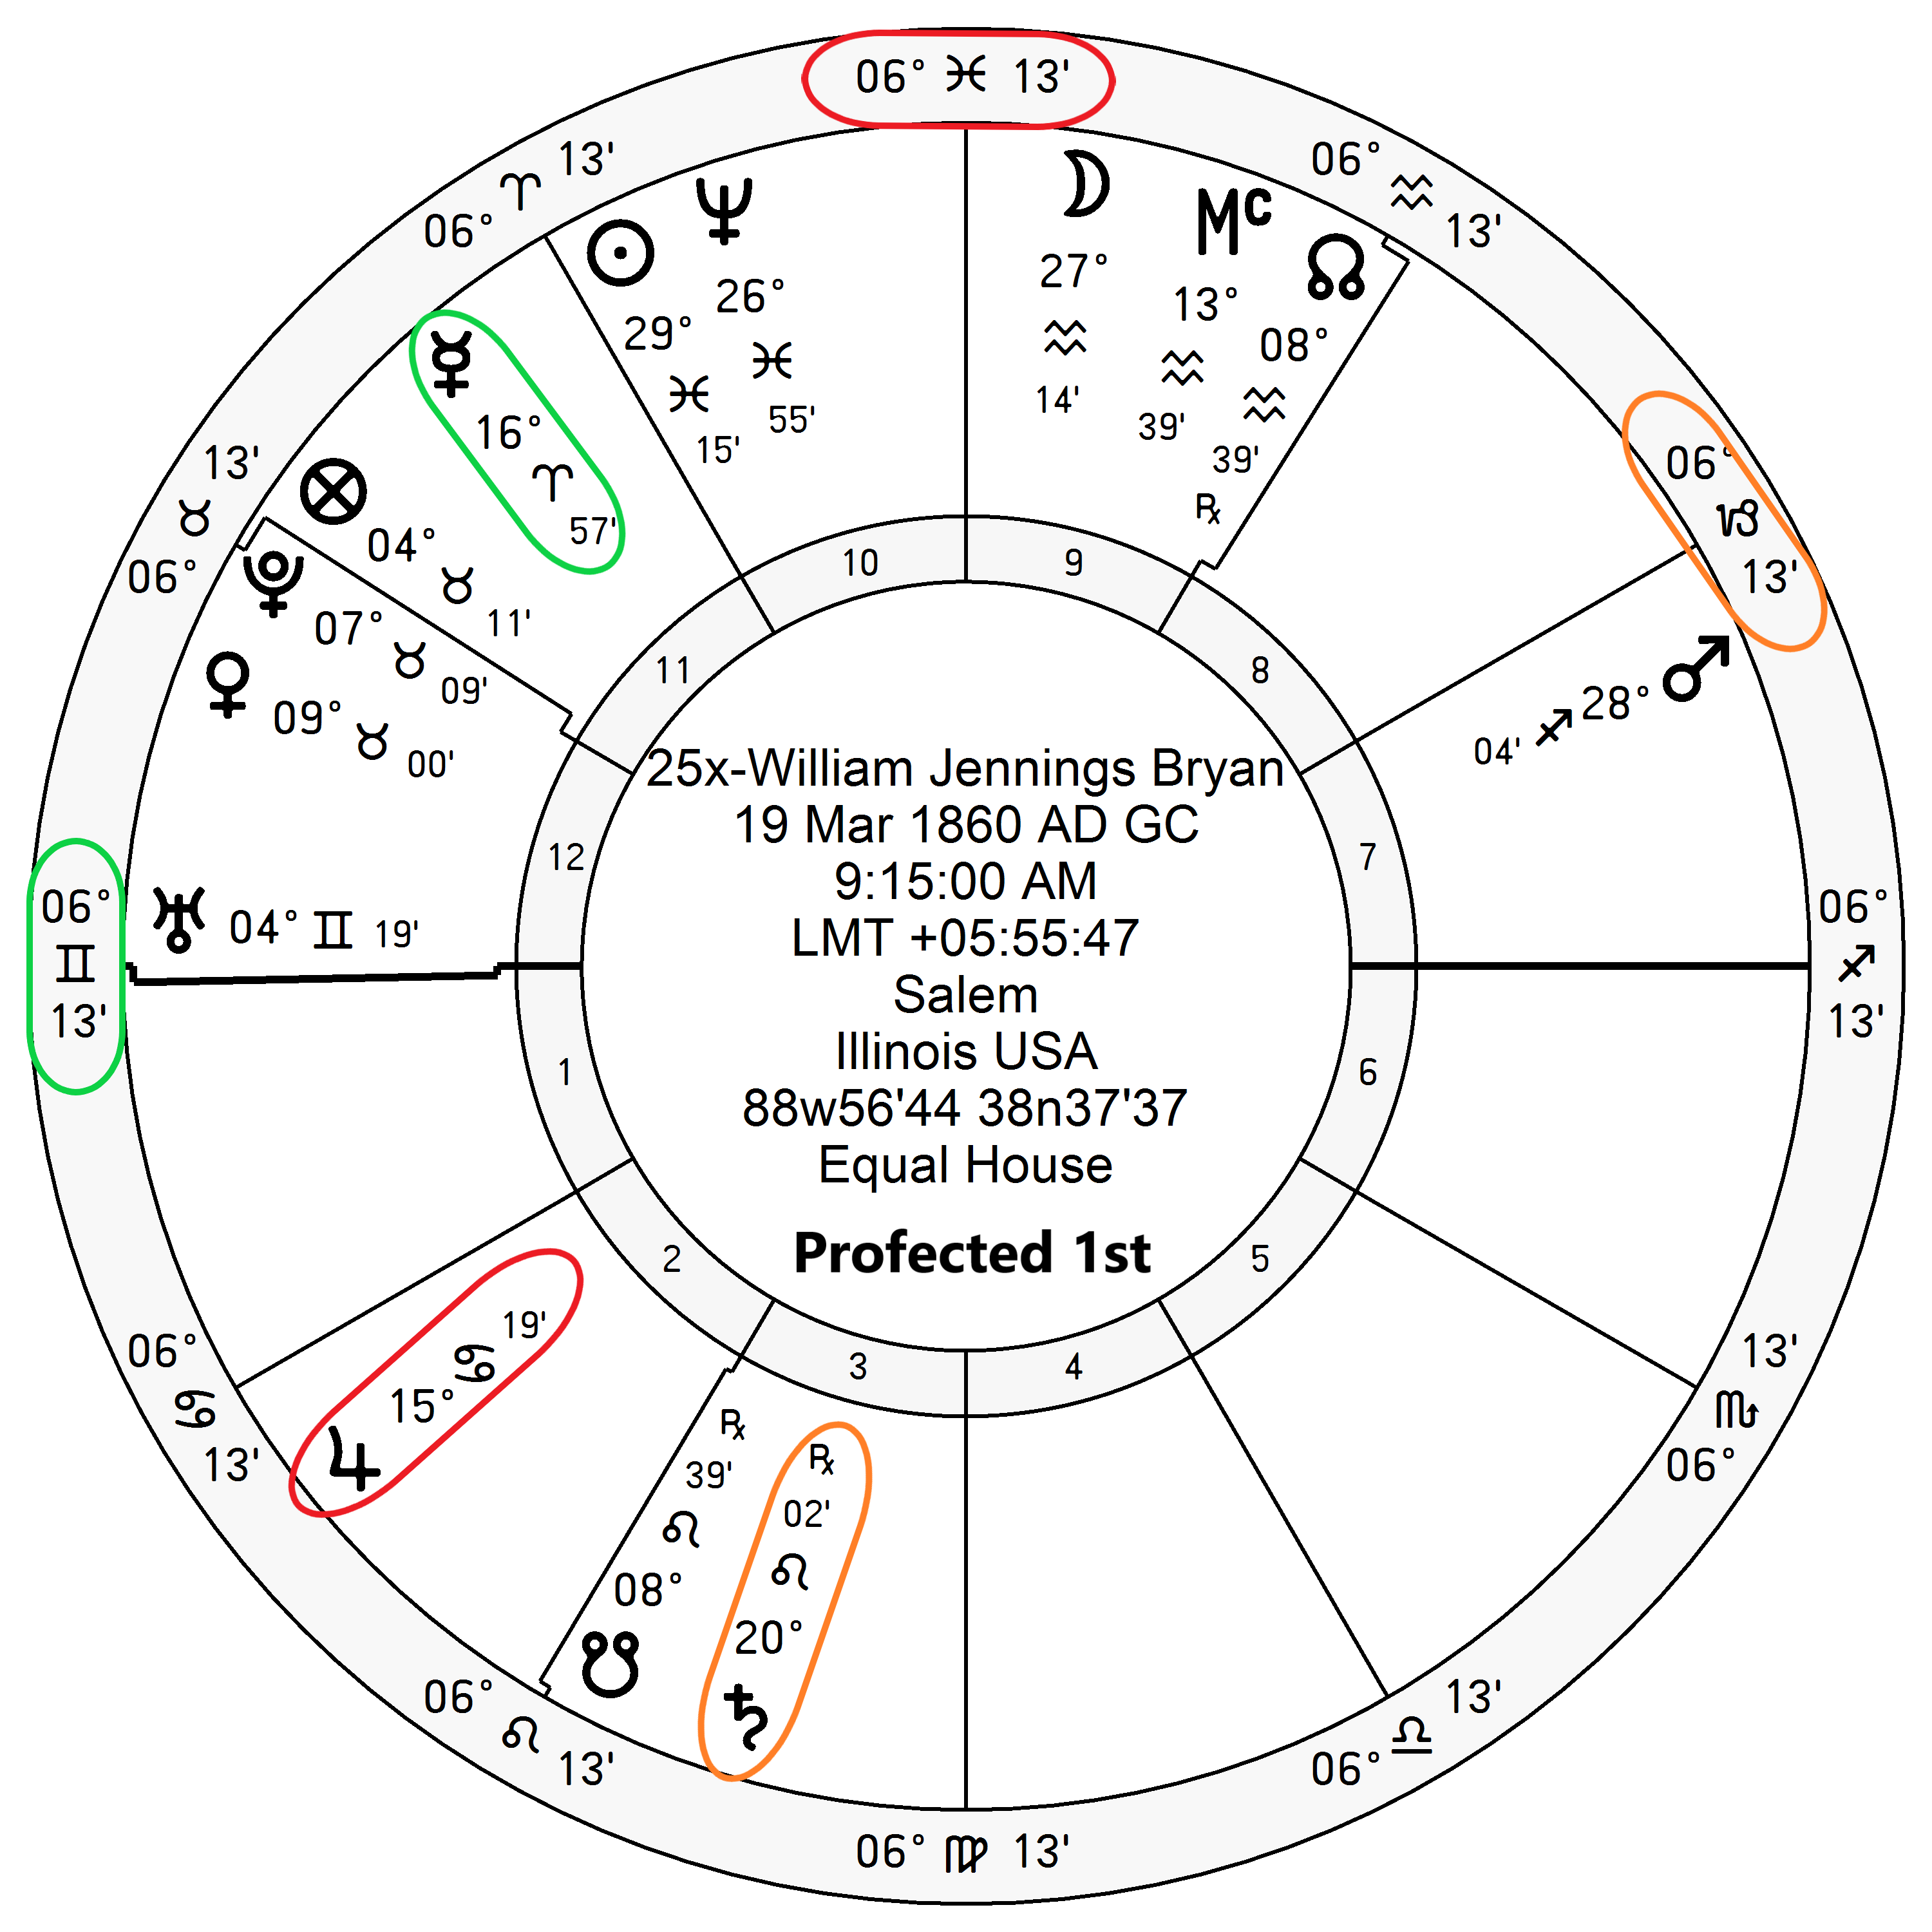
\includegraphics[width=0.9\textwidth]{charts/Bryan-Prof-1st.png}}

\textbf{\dgreen P1=N1} 
	$\Rightarrow$ \Mercury\, $\Rightarrow$ P11/N11\\
\textbf{\red P10=N10}
	$\Rightarrow$ \Jupiter\, $\Rightarrow$ P2/N2\\
PE=P8/N8 
	$\Rightarrow$ \Saturn\,\Retrograde $\Rightarrow$ P3/N4


\end{columns}
\end{frame}
